% file: graph-paths/dijkstra-correctness.tex

\documentclass[tikz]{standalone}
\usepackage{amssymb}

\usetikzlibrary{positioning, shapes, arrows.meta, decorations.pathmorphing, backgrounds, fit}

\begin{document}
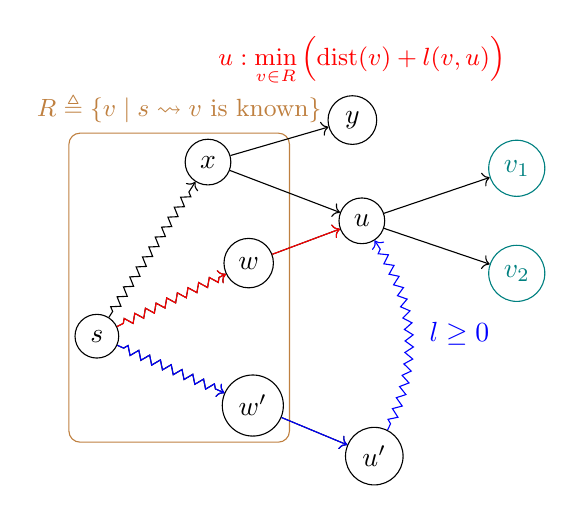
\begin{tikzpicture}[n/.style = {circle, draw}, % node
    leadsto/.style = {->, decorate, decoration = {
    	zigzag, amplitude = 1.50pt, segment length = 1.5mm, pre length = 2.5pt, post length = 2.5pt}},
    e/.style = {->}, % edge
  ]
  % source
  \node (s) [n] {$s$};

  \node (w) [n, above right = 0.5cm and 1.50cm of s] {$w$};
  \node (w') [n, below right = 0.4cm and 1.50cm of s] {$w'$};
  \node (x) [n, above right = 1.8cm and 1.00cm of s] {$x$};

  \path (s) edge[leadsto] (x)
			edge[leadsto] (w)
			edge[leadsto] (w');
  % R
  \node[draw, brown, fit = (s) (x) (w) (w'), rectangle, rounded corners, inner sep = 2pt, 
	label = {[brown, font = \small] above: $R \triangleq \{ v \mid s \leadsto v \textrm{ is known} \}$}] {};

  % \pause
  % R-extension
  \node (u) [n, above right = 0.1cm and 1.00cm of w] {$u$};
  \node (u') [n, below right = 0.1cm and 1.00cm of w'] {$u'$};
  \node (y) [n, above right = 0.1cm and 1.40cm of x] {$y$};

  \path (w) edge[e] (u)
		(w') edge[e] (u')
		(x) edge[e] (y)
			edge[e] (u);

  % \pause
  % s -> w -> u
  \path (s) edge[leadsto, red] (w)
		(w) edge[e, red] (u);
  \node [above = 1.30cm of u, red, font = \small] {$u: \min\limits_{v \in R} \big(\textrm{dist}(v) + l(v,u)\big)$};

  % \pause
  % s -> w' -> u' -> u
  \path (s) edge[leadsto, blue] (w')
		(w') edge[e, blue] (u')
		(u') edge[leadsto, bend right, blue] node [right = 4pt] {$l \ge 0$} (u);

  % \pause
  % update
  \node (v1) [n, above right = 0.20cm and 1.50cm of u, teal] {$v_1$};
  \node (v2) [n, below right = 0.20cm and 1.50cm of u, teal] {$v_2$};

  \path (u) edge[e] (v1)
			edge[e] (v2);
\end{tikzpicture}
\end{document}
